\documentclass{article}


% Use numeric citations (compatible with \bibliographystyle{plain}); nips.sty
% loads natbib in author-year mode by default, which clashes with a numeric .bbl.
\PassOptionsToPackage{numbers, compress}{natbib}


% ready for submission
\usepackage[final]{nips}


% to compile a preprint version, e.g., for submission to arXiv, add add the
% [preprint] option:
%     \usepackage[preprint]{neurips_2025}


% to compile a camera-ready version, add the [final] option, e.g.:
%     \usepackage[final]{neurips_2025}


% to avoid loading the natbib package, add option nonatbib:
%    \usepackage[nonatbib]{neurips_2025}


\usepackage[utf8]{inputenc} % allow utf-8 input
\usepackage[T1]{fontenc}    % use 8-bit T1 fonts
\usepackage{hyperref}       % hyperlinks
\usepackage{url}            % simple URL typesetting
\usepackage{booktabs}       % professional-quality tables
\usepackage{amsfonts}       % blackboard math symbols
\usepackage{nicefrac}       % compact symbols for 1/2, etc.
\usepackage{microtype}      % microtypography
\usepackage{xcolor}         % colors

\usepackage{todonotes}
\usepackage{amsmath}
\usepackage{amsfonts}
\usepackage{graphicx}
\usepackage{color}
\usepackage{listings}
\usepackage{hyperref}
\usepackage{epstopdf}
\usepackage{xparse}
\usepackage{tabulary}
\usepackage{pifont}
\usepackage{algorithm}
\usepackage{algpseudocode}
\usepackage{float}
\usepackage{subcaption}
\usepackage{wrapfig}


\usepackage{amsthm}
\theoremstyle{plain}
\newtheorem{theorem}{Theorem}[section]
\newtheorem{lemma}[theorem]{Lemma}

\theoremstyle{definition}
\newtheorem{definition}{Definition}[section]
\newtheorem{example}[definition]{Example}

\theoremstyle{remark}
\newtheorem{remark}{Remark}[section]


% --- result-number macros (filled from results/summary.csv) ---------------
\newcommand{\cardinalSpeedup}{11}                  % cardinal vs naive expansion ratio (text adds x)
\newcommand{\mlpTopOne}{72\%}                       % MLP imitation top-1 (strong oracle)
\newcommand{\linTopOne}{53\%}                       % linear imitation top-1 (strong oracle)
\newcommand{\numNodes}{2{,}674}                     % training ranking groups
\newcommand{\linHardWin}{geometric-mean expansion ratio as low as $0.48$ (over
$2\times$ fewer expansions) and a per-instance win-rate up to $75\%$ on hard,
dense instances}
\newcommand{\seqFinding}{conditioning on search history did not improve imitation
(best validation top-1 $0.67$, on par with the memoryless models) and did not
reduce expansions over the linear selector in search.}

\title{Learning to Prioritize Conflicts in Conflict-Based Search:\\
A Study of Hand-Crafted and Learned Selection Rules}


% The \author macro works with any number of authors. There are two commands
% used to separate the names and addresses of multiple authors: \And and \AND.
%
% Using \And between authors leaves it to LaTeX to determine where to break the
% lines. Using \AND forces a line break at that point. So, if LaTeX puts 3 of 4
% authors names on the first line, and the last on the second line, try using
% \AND instead of \And before the third author name.


\author{%
  Natalie Pham \\
  \And
  Chaoyang Wang
}
  % \thanks{Use footnote for providing further information
  %   about author (webpage, alternative address)---\emph{not} for acknowledging
  %   funding agencies.} \\
  % Department of Computer Science\\
  % Cranberry-Lemon University\\
  % Pittsburgh, PA 15213 \\
  % \texttt{hippo@cs.cranberry-lemon.edu} \\
  % examples of more authors
  % \And
  % Coauthor \\
  % Affiliation \\
  % Address \\
  % \texttt{email} \\
  % \AND
  % Coauthor \\
  % Affiliation \\
  % Address \\
  % \texttt{email} \\
  % \And
  % Coauthor \\
  % Affiliation \\
  % Address \\
  % \texttt{email} \\
  % \And
  % Coauthor \\
  % Affiliation \\
  % Address \\
  % \texttt{email} \\


\begin{document}
\maketitle
\begin{abstract}
Conflict-Based Search (CBS) is an optimal Multi-Agent Path Finding (MAPF) solver
whose runtime is dominated by a single recurring choice at every high-level node:
which conflict to branch on. We build an optimal CBS with a pluggable
conflict-selection interface and ask whether a learned selector can outperform
the standard \emph{cardinal} heuristic. On random grids the selection rule
changes high-level expansions by up to an order of magnitude. We define a
subtree-minimizing oracle that is a one-step policy improvement over cardinal
and, following Huang et al.\ \cite{Huang2020resolveconflictsforMAPF}, train a
linear ranker and an MLP to imitate it. The linear ranker beats cardinal on hard
instances (per-instance geometric-mean expansion ratio as low as $0.48$ and
win-rate up to $75\%$); the advantage grows with agent and obstacle density,
transfers to unseen $10\times10$ and $12\times12$ grids, and survives in
wall-clock time, while solution cost remains optimal. The linear model also
beats the MLP, which overfits the oracle. Learned focal node ordering in
bounded-suboptimal ECBS and a GRU over the search history do not robustly
improve over their baselines, consistent with conflict selection being
near-Markovian in the current MDD features. Code and models are released.
\end{abstract}
\vspace{-18pt}
\section{Introduction}
\vspace{-8pt}
Multi-Agent Path Finding (MAPF) asks for collision-free paths that route a team
of agents from their starts to their goals at minimum total cost. It underpins
automated warehouses, traffic, and multi-robot systems. Conflict-Based Search
(CBS) \cite{sharon2015conflict} solves MAPF optimally by a two-level search: a
low level plans single-agent paths under constraints, and a high level resolves
inter-agent collisions by branching. The high-level \emph{constraint tree} can
grow exponentially with agent interactions, and in practice its size is governed
by one design choice made at every node: \emph{which conflict to resolve first}.

The classic hand-crafted answer is to prefer \emph{cardinal} conflicts---those
that provably increase cost on both branches \cite{boyarski2015icbs}. Huang,
Koenig \& Dilkina \cite{Huang2020resolveconflictsforMAPF} instead \emph{learn} a
conflict-selection rule by imitating an expensive oracle with a linear ranking
function. We take conflict prioritization as our object of study and ask three
questions: \textbf{(RQ1)} how much does the selection rule matter?
\textbf{(RQ2)} can a lightweight learned ranker match or beat the best
hand-crafted rule? \textbf{(RQ3)} in which density regimes does CBS begin to
fail, and does prioritization shift that frontier?

\noindent\textbf{Contributions.}
(1) An optimal CBS and a bounded-suboptimal ECBS with MDD-based cardinality and
a pluggable selection interface.
(2) An empirical characterization of conflict prioritization across agent and
obstacle densities, isolating search effort because cost is held optimal.
(3) A subtree-minimizing policy-improvement oracle and a learned linear selector
that imitates it and beats cardinal on hard instances (per-instance geometric-
mean expansion ratio down to $\sim\!0.5$, win-rate up to $75\%$), with the gain
growing with difficulty and transferring to larger unseen grids; the linear model
beats an MLP that overfits the oracle.
(4) Two negative results: learned focal ordering in ECBS and a search-history
sequence model, both pointing to conflict selection being near-Markovian.
\vspace{-10pt}
\section{Related works}
\vspace{-10pt}
\textbf{Classical MAPF. }CBS \cite{sharon2015conflict} decomposes MAPF into high-level conflict resolution and low-level single-agent planning, with completeness and optimality. Its complexity grows rapidly in dense environments. Enhanced CBS \cite{barer2014suboptimal} and ICBS \cite{boyarski2015icbs} introduced bounded-suboptimal search and improved conflict prioritization. These rely on hand-crafted heuristics over local conflict statistics.

\textbf{Learning-based MAPF. }A separate line learns decentralized neural policies for MAPF, trading correctness guarantees for scale. We instead keep CBS exact and learn only the conflict-selection policy.

\textbf{Learned conflict selection. }Most directly related to our work, Huang, Koenig \& Dilkina \cite{Huang2020resolveconflictsforMAPF} keep CBS exact but replace its hand-crafted conflict-selection rule with a learned one. They define an oracle that selects the conflict yielding the smallest constraint-tree subtree; because the oracle is too expensive to run online, they train a \emph{linear ranking function} by imitation learning to reproduce its choices from cheap per-conflict features, reporting improved success rates, smaller search trees, and faster runtimes. Our study reproduces and extends this recipe at small scale: a cheaper subtree-minimizing oracle (a one-step policy improvement over cardinal) and both linear and MLP rankers, used to bridge the hand-crafted cardinal heuristic and a learned alternative that surpasses it.

\textbf{Sequence models. }State-space sequence models such as Mamba \cite{gu2023mamba} motivate one of our exploratory directions: conditioning conflict selection on the history of conflicts resolved along a root-to-node path. We treat this as a hypothesis to test rather than a method assumed to work.
\vspace{-10pt}
\section{Method}
\vspace{-6pt}

\textbf{Problem and CBS.} A MAPF instance is a 4-connected grid, a set of $k$
agents each with a start and goal, and discrete time; each step an agent moves to
an adjacent cell or waits. A solution is collision-free if no two agents share a
cell (\emph{vertex} conflict) or swap across an edge (\emph{edge} conflict) at the
same time, and we minimize sum-of-costs (SOC). CBS \cite{sharon2015conflict}
searches a binary \emph{constraint tree}: each node holds a constraint set and the
per-agent paths obtained by a low-level space-time A$^\ast$ respecting those
constraints. If the joint plan has conflicts, CBS picks one conflict
$\langle a_i,a_j,\text{loc},t\rangle$ and creates two children, each forbidding one
agent from the conflicting move; the affected agent is replanned. Expanding the
high level in best-first order of SOC yields an optimal solution. Crucially, the
\emph{choice of which conflict to branch on} affects only the size of the tree,
not the returned cost---so every selection strategy we compare is optimal and
differs only in search effort.

\textbf{Conflict cardinality.} For each agent we build a Multi-valued Decision
Diagram (MDD): the union of all constraint-respecting optimal paths of its current
cost. The \emph{width} of the MDD at level $t$ is how many cells the agent could
occupy at time $t$. A vertex conflict at $(v,t)$ is \emph{cardinal} if both agents
have width $1$ at $t$ (both are forced through $v$, so resolving it raises cost on
both children), \emph{semi-cardinal} if exactly one is forced, and
\emph{non-cardinal} otherwise \cite{boyarski2015icbs}. Resolving cardinal
conflicts first is the standard heuristic that makes CBS practical.

\textbf{Hand-crafted selectors.} We implement five strategies behind one
interface: \texttt{first} (the first conflict found, i.e.\ naive CBS),
\texttt{random}, \texttt{earliest} (smallest $t$), \texttt{most-conflicts} (a
degree heuristic preferring conflicts whose agents appear in many conflicts), and
\texttt{cardinal} (cardinal\,$\succ$\,semi\,$\succ$\,non, ties broken by earliest
$t$)---the strong ICBS baseline.

\textbf{Oracle and learned selectors.} Following
\cite{Huang2020resolveconflictsforMAPF}, we learn a selector by imitating an
oracle. The oracle is a one-step policy improvement over cardinal: at a node, for
each candidate conflict we branch on it and measure the resulting subtree size
when it is solved as a whole with cardinal as the rollout policy, then pick the
conflict minimizing this size. Because cardinal's own choice is among the
candidates, the oracle expands no more nodes than cardinal at every node, giving
a target that can exceed it. The cost must be measured on the subtree explored as
a whole (best-first, early-stopping); summing the two child subtrees solved in
isolation mis-ranks conflicts and in our experiments underperforms cardinal. The
oracle is too expensive to run online (it rolls out subtrees), motivating a
learned approximation. Running oracle-guided CBS yields, at each node, a feature
matrix over its conflicts and the oracle's chosen index. Each conflict is
represented by a $24$-dimensional vector: type; timing; both agents' MDD widths
at $t{-}1,t,t{+}1$ and singleton flags; cardinality one-hot; path costs and
remaining distance-to-goal at the conflict cell; per-agent conflict degree; and
the node's total conflict count. We train two memoryless rankers by listwise
softmax cross-entropy with the oracle's choice as the positive class: a linear
ranker and a one-hidden-layer MLP (32 tanh units), both in numpy with Adam.

\textbf{Sequence model.} To test whether search history helps, we attach to each
node the sequence of feature vectors of the conflicts its ancestors resolved and
train a GRU to score the current node's conflicts conditioned on that history,
again by imitation of the oracle. This is the only component using PyTorch.

\textbf{Bounded-suboptimal ECBS and learned focal ordering.} We also study the
bounded-suboptimal regime (ECBS \cite{barer2014suboptimal}). With an optimal low
level, a node's cost lower-bounds any solution under its constraints; high-level
focal search expands, among nodes with cost $\le w\cdot\min\text{-cost}$, the one
chosen by a pluggable node selector, guaranteeing solutions within $w\times$
optimal. The standard rule orders by fewest conflicts; we instead learn to
predict whether a node lies on the path to a solution, from cheap node-level
features (conflict counts and types, cost, depth, agent-conflict degree, conflict
timing), labelled by recovering the solution node's ancestors.

\vspace{-4pt}
\section{Experimental setup}
\vspace{-6pt}
All experiments use random $8\times8$ 4-connected grids with obstacle densities
$\{0,0.1,0.2\}$ and varying agent counts $k$, with goals reachable from starts.
The hand-crafted comparison sweeps $k\in\{4,\dots,14\}$ over $20$ seeds within a
$6$\,s / $3000$-node budget. The learned-vs-cardinal comparison uses a larger
sweep ($k\in\{6,8,10,12,14\}$, $80$ seeds, $10$\,s / $8000$-node budget). We
report high-level expansions, runtime, and success rate; solution cost is logged
as a correctness check (identical across strategies). Expansion counts are
heavy-tailed, so we compare learned methods to cardinal by the per-instance
expansion ratio on commonly-solved instances, reporting its median, geometric
mean, and win-rate. Training data is the oracle's choices on \numNodes{}
multi-conflict nodes from a disjoint seed range; reported results are on held-out
instances.

\section{Results \& Analysis}
\vspace{-6pt}

\begin{figure}[t]
  \centering
  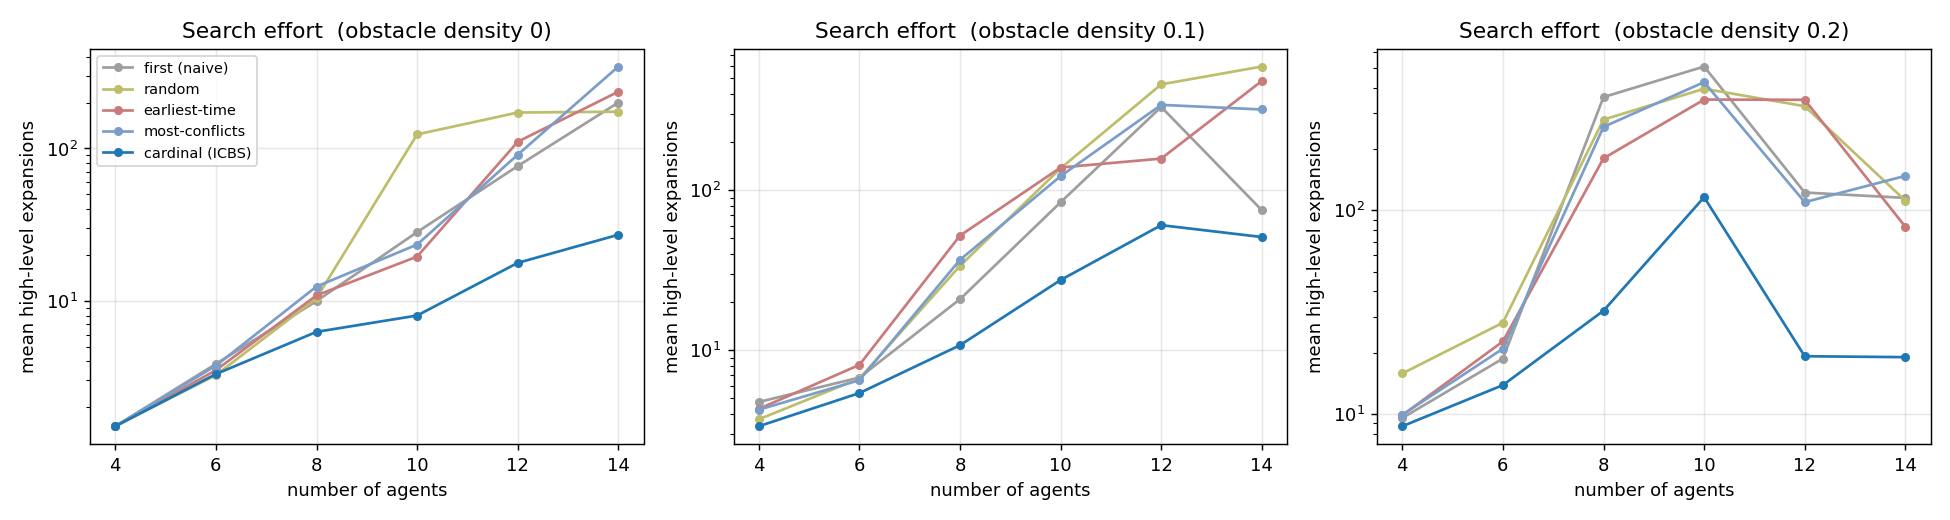
\includegraphics[width=\linewidth]{figures/fig_expansions.png}
  \vspace{-16pt}
  \caption{High-level node expansions vs.\ number of agents (log scale), one
  panel per obstacle density, averaged over instances solved by all strategies.
  The cardinal heuristic and the learned rankers expand far fewer nodes than
  naive selection; the gap widens with agent density.}
  \label{fig:expansions}
  \vspace{-10pt}
\end{figure}

\begin{figure}[t]
  \centering
  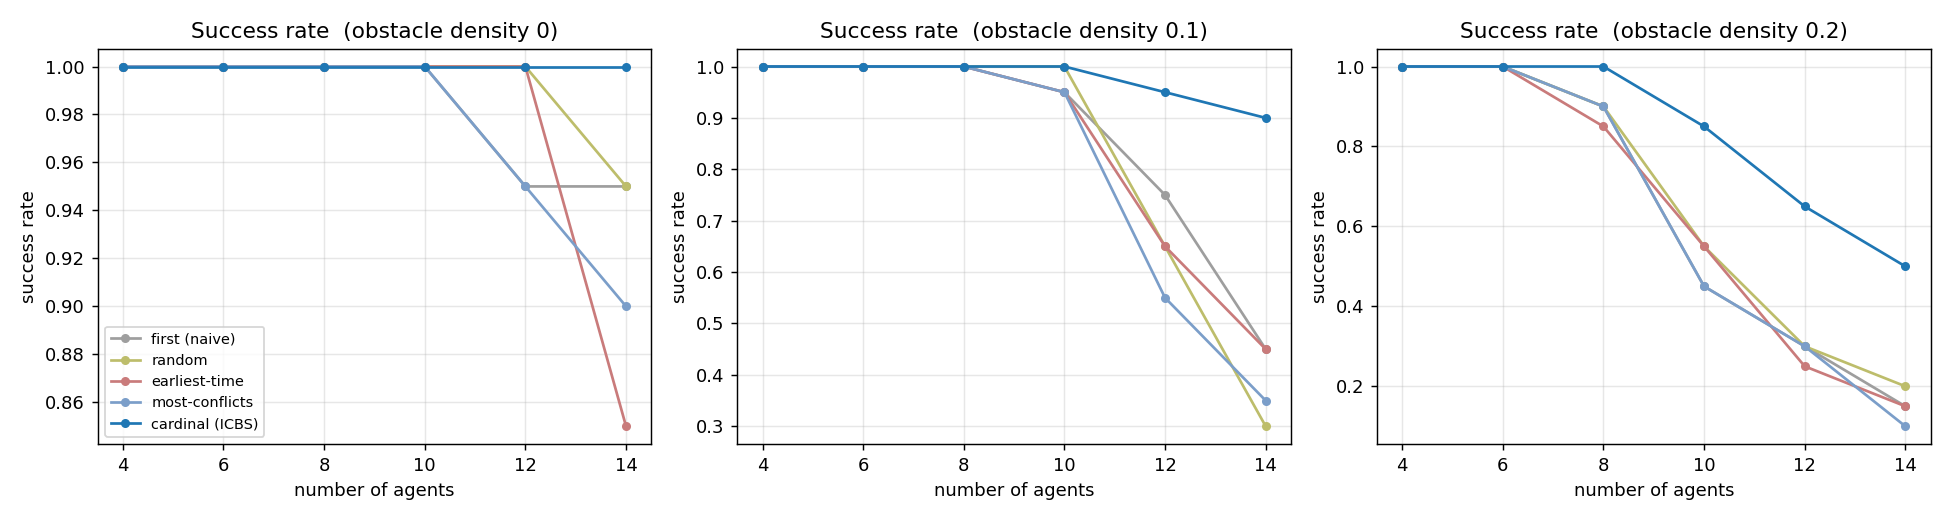
\includegraphics[width=\linewidth]{figures/fig_success.png}
  \vspace{-16pt}
  \caption{Success rate within the $6$\,s / $3000$-node budget. Better
  prioritization pushes the failure frontier to higher agent counts.}
  \label{fig:success}
  \vspace{-12pt}
\end{figure}

\textbf{RQ1: prioritization matters by up to an order of magnitude.}
Figure~\ref{fig:expansions} shows that on easy instances all strategies are
indistinguishable, but as the number of agents grows the constraint tree
explodes for naive selection while staying small for cardinal. At the densest
solved-by-all cells, \texttt{cardinal} expands roughly $\cardinalSpeedup\times$
fewer high-level nodes than \texttt{first}, with a correspondingly large runtime
gap. Picking the \texttt{earliest} conflict in time is often \emph{worse} than
picking an arbitrary first conflict, because early conflicts are frequently
non-cardinal and resolving them fails to prune the tree: the content of a
conflict (whether it forces a cost increase), not its position, is what matters.

\begin{figure}[t]
  \centering
  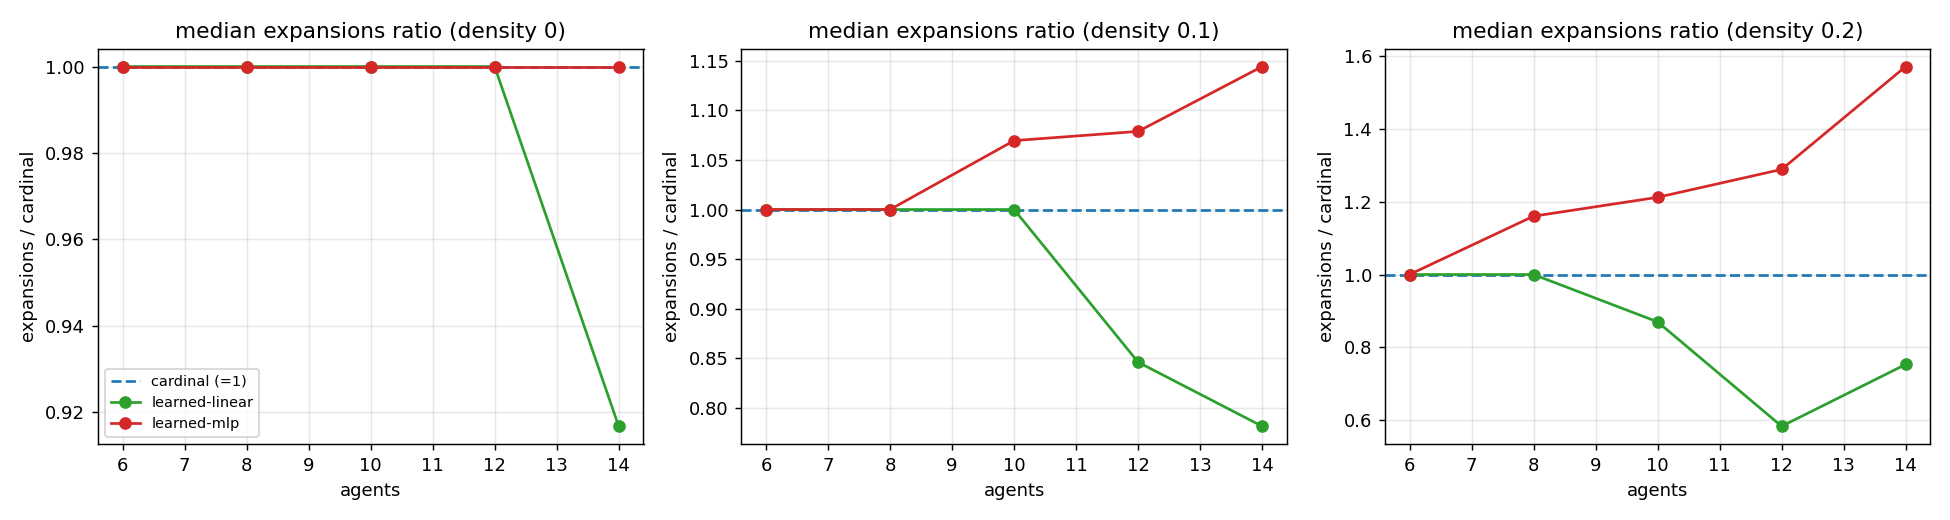
\includegraphics[width=\linewidth]{figures/fig_learned_ratio.png}
  \vspace{-16pt}
  \caption{Median per-instance expansion ratio of the learned selectors to
  cardinal (lower is better; the dashed line is cardinal). On easy instances all
  match cardinal (ties); the \emph{linear} selector increasingly beats cardinal as
  instances get harder, while the MLP overfits the oracle and does not.}
  \label{fig:ratio}
  \vspace{-12pt}
\end{figure}

\textbf{RQ2: a learned linear selector beats cardinal on hard instances.}
The oracle itself is a real improvement over cardinal: oracle-guided CBS expands
$0.74$--$0.86\times$ as many nodes as cardinal at 8--9 agents with an adequate
rollout budget. Trained to imitate it, the linear ranker reaches \linTopOne{} and
the MLP \mlpTopOne{} top-1 agreement. In search (Fig.~\ref{fig:ratio}), the two
learned selectors tie cardinal on easy instances (same tiny trees), but as agents
increase the linear ranker pulls ahead: \linHardWin{}, with the advantage growing
monotonically with difficulty. Because every strategy is optimal, solution cost
is identical, so this is pure search-effort saving on the hard instances. The
linear model beats the MLP despite lower imitation accuracy ($53\%$ vs $72\%$):
the MLP overfits the oracle's idiosyncratic choices while the linear model
captures the signal that transfers to held-out instances. A feature ablation
isolates the mechanism: a ranker using only MDD/cardinality features (widths,
singleton flags, cardinality one-hot) matches the full model's held-out top-1
($0.55$), removing them drops it to $0.45$, and cost/distance/timing features
alone reach only $0.41$. The learned rule therefore keeps cardinal's core signal
but uses the continuous MDD widths to break ties among cardinal conflicts more
finely than cardinal's categorical, earliest-time rule.

\begin{table}[t]
\centering\small
\caption{Per-instance expansion ratio of the learned \emph{linear} selector to
cardinal in optimal CBS (geometric mean; win-rate, the fraction of instances with
ratio${<}1$, in parentheses), on held-out instances ($80$ seeds/cell). Below $1$
means fewer expansions than cardinal. The advantage grows with both agent count
and obstacle density; the MLP (omitted) stays ${\ge}1$ throughout.}
\label{tab:rq2}
\begin{tabular}{lccc}
\toprule
agents & density $0$ & density $0.1$ & density $0.2$ \\
\midrule
8  & 0.98 (15\%) & 0.96 (20\%) & 0.86 (41\%) \\
10 & 0.93 (28\%) & 0.87 (42\%) & 0.68 (62\%) \\
12 & 0.82 (45\%) & 0.70 (62\%) & \textbf{0.48 (75\%)} \\
14 & 0.80 (58\%) & 0.60 (70\%) & 0.61 (70\%) \\
\bottomrule
\end{tabular}
\end{table}

\textbf{Generalization and runtime.} The selector is trained only on $8\times8$
grids. On unseen larger grids it generalizes, and the advantage is if anything
larger: at density $0.2$ and $14$ agents the geometric-mean expansion ratio is
$0.38$ on $10\times10$ and $0.47$ on $12\times12$, with win-rates of $74$--$84\%$.
The gain survives in wall-clock time despite per-node inference; on those hard
cells the runtime ratio reaches $\sim\!0.44$, because the linear features reuse
the MDDs cardinal already builds. The only cost is on easy instances, where
inference adds a $\sim\!5$--$10\%$ overhead with no expansions to save; falling
back to cardinal until the tree grows beyond a few nodes removes it. Fewer
expansions also let more instances finish within the budget: at density $0.2$
and $14$ agents the linear selector raises success rate to $56\%$ vs cardinal's
$38\%$ on $8\times8$, $75\%$ vs $62\%$ on $10\times10$, and $90\%$ vs $77\%$ on
$12\times12$; the overfit MLP solves fewer than cardinal.

\textbf{Two further directions did not robustly improve.} (i)~\emph{Learned
focal ordering in ECBS}: a classifier predicting whether a node lies on a
solution path, used as focal priority. Pure learned ordering is high-variance and
not reliably better than fewest-conflicts (median ratio $\approx1.0$--$1.6$, with
occasional blow-ups and a lower success rate on hard instances); a blended
variant that uses the learned score only to break ties is stable but at best on
par. (ii)~A sequence model (GRU over the root-to-node history of resolved
conflicts): \seqFinding{} Both findings are consistent with conflict selection
being near-Markovian in the current node's MDD features.

\textbf{RQ3: the failure frontier.} Figure~\ref{fig:success} characterizes when
CBS stops solving instances within budget. Success rate degrades with both agent
count and obstacle density, but the rate of degradation depends strongly on the
selection rule: naive strategies fall off first, while cardinal and the learned
rankers sustain high success rates to substantially larger agent counts. In
other words, conflict prioritization does not merely speed up easy instances---it
shifts the boundary of what is solvable at all under a fixed budget.

\vspace{-4pt}
\section{Discussion}
\vspace{-6pt}
Two implementation choices were important. First, the oracle must score a choice
by the cost of solving the subtree as a whole under best-first early-stopping;
an initial version that summed isolated child subtrees was actually worse than
cardinal. Second, a linear ranker generalised better than the MLP despite lower
training-imitation accuracy, because the MLP overfit the oracle's idiosyncrasies.
The optimality invariant (identical solution cost across all strategies on every
solved instance) is evidence the solver is correctly implemented.

Two further directions did not robustly improve on their baselines. Learned
focal ordering for ECBS was high-variance: an on-path classifier is a poor
stand-alone priority because the on-path signal is sparse and policy-dependent,
so the model occasionally dives into dead-end branches. A sequence model over
the search history did not beat the memoryless linear selector, and its
imitation accuracy was no higher. Both findings indicate that CBS conflict
selection is close to Markovian in the current node's MDD features. One
methodological note: expansion counts are heavy-tailed and ratio-of-means can
mislead (we initially saw an illusory $3\times$ focal speed-up); per-instance
medians and win-rates are needed. A follow-up policy-improvement step ---
using the learned linear as the oracle's rollout policy with a larger subtree
budget --- produces a second linear that beats the one in Table~\ref{tab:rq2}
by $8$--$14\%$ per-instance geomean on the same hard cells; higher-capacity
models (MLP, GNN over the conflict graph) and richer features did not, so the
model is at the ceiling and the oracle is the bottleneck.

\textbf{Limitations.} Our pure-Python solver restricts us to small grids;
absolute runtimes are not comparable to optimised C++ solvers, though expansion
counts are. The oracle is a one-step policy improvement over cardinal, not the
globally optimal selection policy, so the learned ceiling we report is
conservative. On a structured $4$-rooms map the learned selector does not
underperform cardinal but its edge narrows to roughly par. A faster solver would
enable MovingAI-scale benchmarks and richer models.

\vspace{-6pt}
We studied conflict prioritization in CBS by isolating it as the single variable
on an optimal solver. Prioritization changes search effort by up to an order of
magnitude and shifts the solvability frontier. A linear selector trained to
imitate a subtree-minimizing oracle beats the cardinal heuristic on hard
instances (\linHardWin{}), with the advantage growing with difficulty and
transferring to unseen larger grids, while solution cost remains optimal. Learned
focal ordering in ECBS and a search-history sequence model do not robustly
improve over their baselines, indicating that conflict selection is near-Markovian
in the current node's MDD features. Code and models are released.

% \section{Possible failures of the proposed idea}
% \vspace{-10pt}
% Although integrating Mamba/S4 with CBS is promising, several challenges may limit its effectiveness. CBS conflict sequences may not exhibits predictable temporal structure for sequence modeling to improve branching decisions, and repeated neural inference may offset search efficiency gains, especially in dense MAPF instances. In such cases, we are also interested in analyzing the negative results, which could provide valuable insight into the limitations of sequence models for symbolic planning and whether long-range temporal modeling can effectively guide combinatorial MAPF search. Since the proposed approach depends on learning from CBS search trajectories, collecting sufficiently diverse conflict sequences may require solving many difficult MAPF instances offline.

\bibliographystyle{plain}
\bibliography{ref}




\end{document}
